% Report schematic (not an experimental result).
% Contrasts a naive row-wise random split of image observations against
% a specimen-level grouped split, for four illustrative specimens A-D
% each with several repeated image observations.
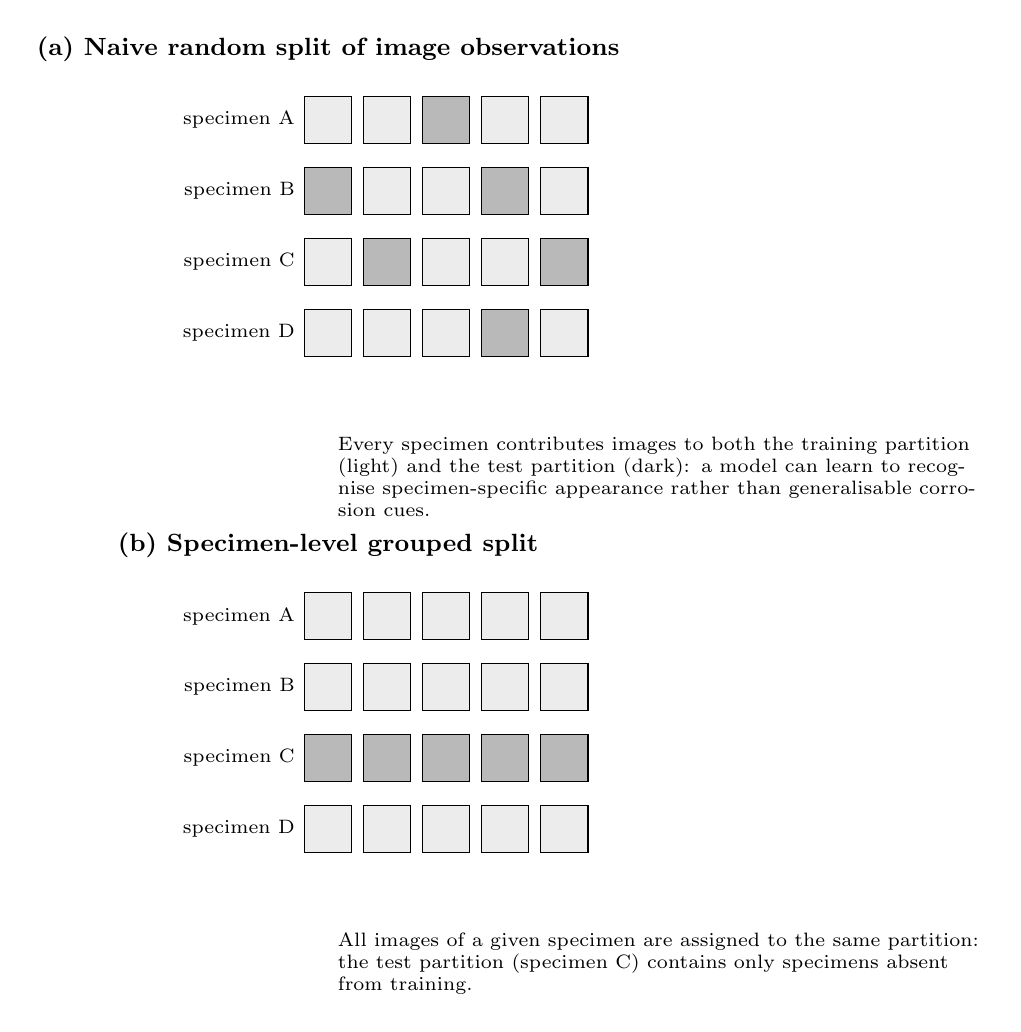
\begin{tikzpicture}[
    sq/.style={draw, minimum size=6mm, inner sep=0pt, font=\tiny},
    train/.style={sq, fill=gray!15},
    test/.style={sq, fill=gray!55},
    lbl/.style={font=\scriptsize, anchor=east},
    panelcap/.style={font=\small\bfseries}
]

% --- Panel (a): naive random row-wise split ---
\node[panelcap] at (0,0) {(a) Naive random split of image observations};

\foreach \row/\name/\pattern [count=\r from 0] in
    {0/A/{train,train,test,train,train},
     1/B/{test,train,train,test,train},
     2/C/{train,test,train,train,test},
     3/D/{train,train,train,test,train}} {
    \node[lbl] at (-0.3,-0.9-\r*0.9) {specimen \name};
    \foreach \p [count=\c from 0] in \pattern {
        \node[\p] at (\c*0.75,-0.9-\r*0.9) {};
    }
}
\node[font=\scriptsize, align=left, text width=8.2cm, anchor=north west]
    at (0,-4.8) {Every specimen contributes images to both the training
    partition (light) and the test partition (dark): a model can learn to
    recognise specimen-specific appearance rather than generalisable
    corrosion cues.};

% --- Panel (b): specimen-level grouped split ---
\begin{scope}[yshift=-6.3cm]
\node[panelcap] at (0,0) {(b) Specimen-level grouped split};

\foreach \row/\name/\assign [count=\r from 0] in
    {0/A/train,1/B/train,2/C/test,3/D/train} {
    \node[lbl] at (-0.3,-0.9-\r*0.9) {specimen \name};
    \foreach \c in {0,...,4} {
        \node[\assign] at (\c*0.75,-0.9-\r*0.9) {};
    }
}
\node[font=\scriptsize, align=left, text width=8.2cm, anchor=north west]
    at (0,-4.8) {All images of a given specimen are assigned to the same
    partition: the test partition (specimen C) contains only specimens
    absent from training.};
\end{scope}

\end{tikzpicture}
